\section{Comportment d'une couche limlite}

Quand un fluide entre en contact avec un solide, on parle d'écoulements pariétaux. La parois d'un solide a une forte influence sur le phenomene la turbulence qui s'y developpe. Ainsi dans ce chapitre il est necessaire de présenté les propriété de ces ecoulement avant de discuté de leur modélisation avec des artefact numerique que sont les lois de parois.

\subsection{Nombre de reynold}

La premieres expérience qui a mis en evidence le phenomene de turbulence à eu lieu à la fin du 19eme siecle par  Osborne Reynolds. Il decida d'etudier l'ecoulement d'un liquide coloré dans un conduit cylindrique. Il constate que à faible vitesse l'ecoulement omet aucune instabilité et reste parallele à la paroi, l'ecoulement est  dit laminaire. En augmentant la vitesse de facon progressive du liquide, le filet coloré commence à devnenir instable à certain endroit, il observe des ecoulemnts regulier et instables dans la conduite cylindrique, l'écoulement est defini comme transitoire. A vitesse élevé l'écoulement devient irregulier et déshorganisé, on considére alors l'ecoulement turbulent. Ces régimes d'écoulement sont caracterisés avec le nombre de Reynold, une grandeur adimensionné, définit par:

$$R_e=U_eL/\nu$$

Avec L la longueure caractéristique et $U_e$ la vitesse de caractéristique de l'écoulement, $\nu$ est la viscosité cinématique du fluide. Ce nombre adimensionné represente le rapport entre les forces innertielles et visqueuses. Il permet de définir le regime d'un ecoulement cité au-dessus. Pour des nombre de Raynold petit on parlera alors de regime laminaire et pour des nombre de Reynold élevé les écoulement seront turbulents.

\begin{figure}[!ht]
 \centering
 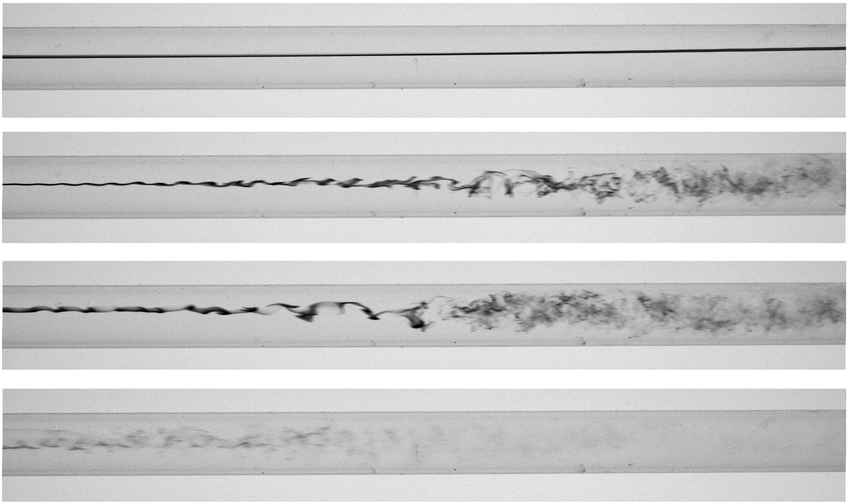
\includegraphics[width=0.7\linewidth]{chapter5_wall_models/pictures/reynold.png}
 \vspace{-2ex}
 \caption{IXV spatial navette by esa}
  \vspace{2ex}
 \label{chap1}
\end{figure}

En présence d'écoulement pariétaux, une zone tres fine est affecté par la paroi, nommée couche limite. Cette zone représente est la région de transition entre la paroi où la vitesse est nulle et la région lointaine où la vitesse du fluide est homogène, que l’on appelle vitesse extérieure et que l’on note $U_\infty$. Les prémieres études theorique sur des plaque planes (ref (Schlichting et Gersten) ont permis de déterminer le regime d'une couche limite en fonction du nombre de Reynold construit selon la position longitdinal d'un corp notée x. Pour un $x=x_{crit}$ on peut définir un nomre de Reynold critique:

$$Re_x=\left(\frac{U_{\infty}x}{\nu}\right)$$

$$Re_{crit}=\left(\frac{U_{\infty}x_{crit}}{\nu}\right)$$

La limite en le regime turbulent et laminaire est atteinte pour un $Re_{crit} \approx 10^2$. Ainsi pour un nombre de Reynold $Re_x > Re_{crit}$ la couche limite, dans le cas contraire elle est considére laminaire. Ainsi pour des écoulement hypersonique les couches limites seront turbulentes.
\begin{figure}[!ht]
 \centering
 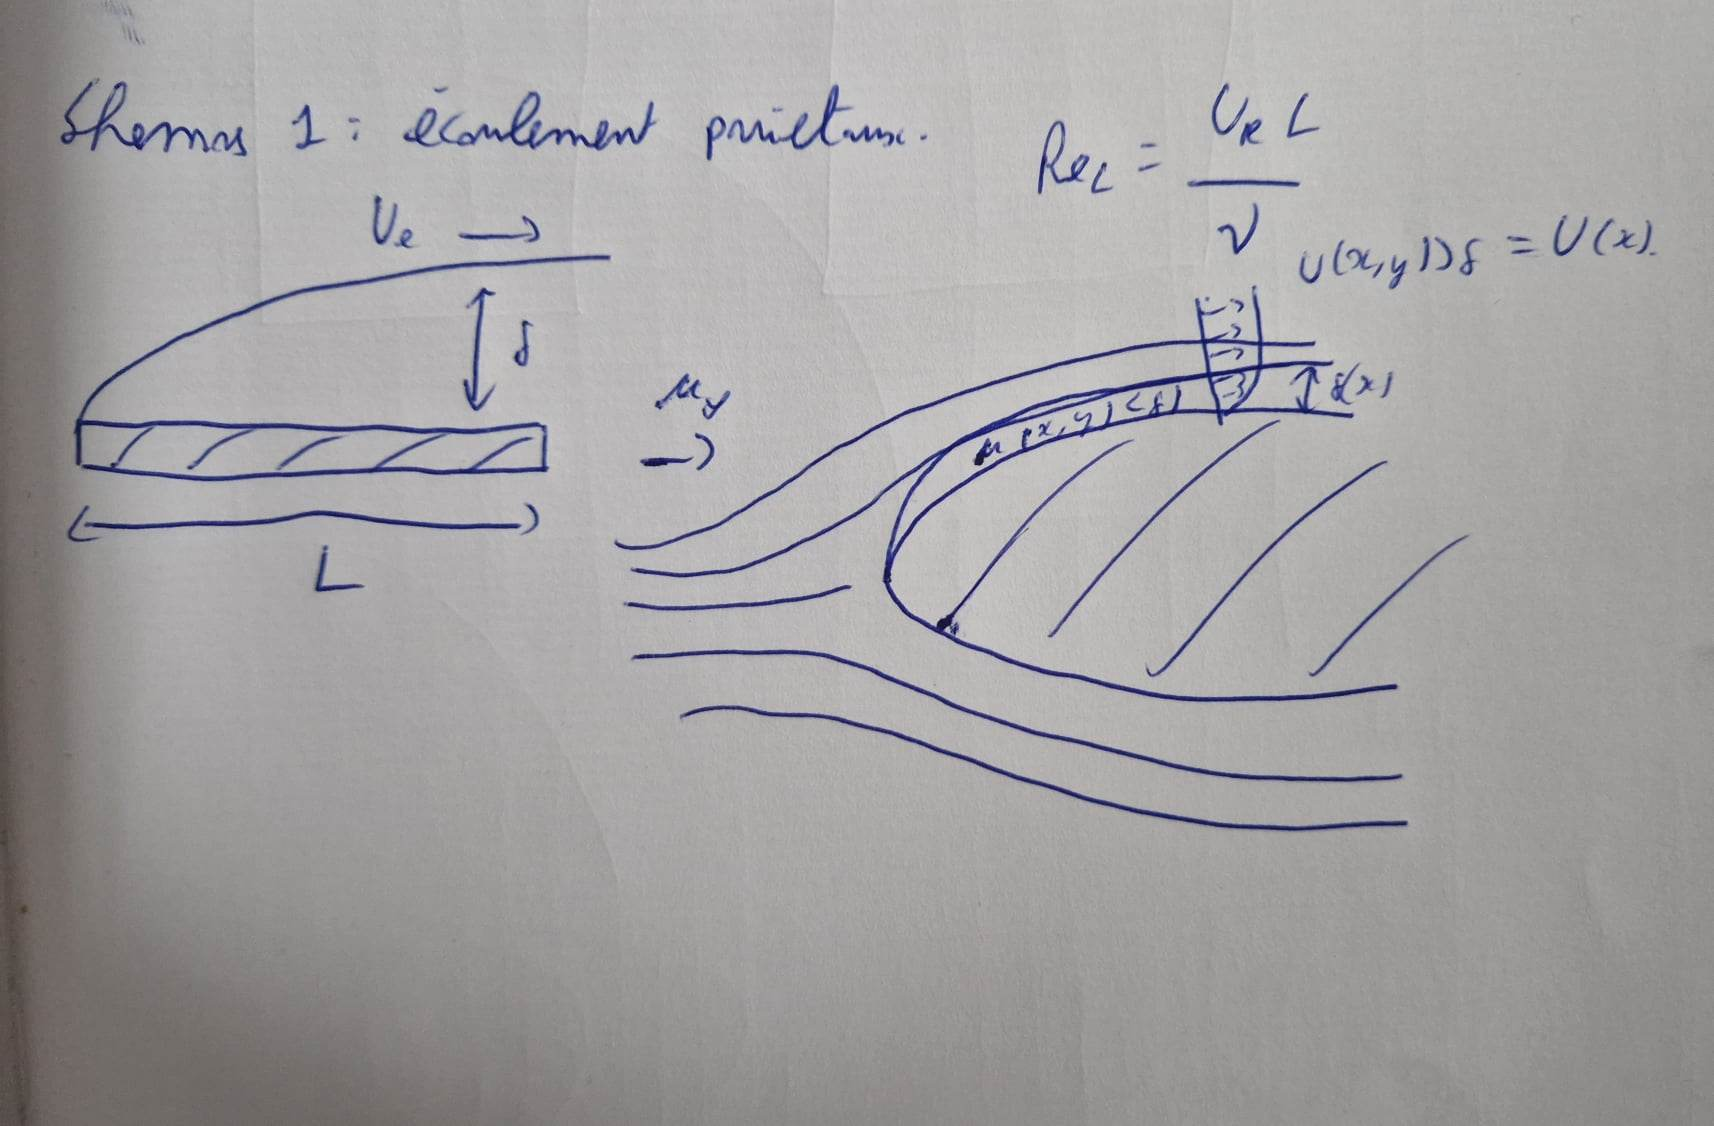
\includegraphics[width=0.7\linewidth]{chapter5_wall_models/pictures/wm1.jpg}
 \vspace{-2ex}
 \caption{IXV spatial navette by esa}
  \vspace{2ex}
 \label{chap1}
\end{figure}

\subsection{Equation d'une couche Limite et description}
\subsection{Pourquoi utilisé une loi de paroi}
